%!TEX root = ../thesis.tex
\section{Analysis of the one-dimensional model assumptions\label{sec:1D_assumptions}}
In constructing our one-dimensional foraging model, there were a number of assumptions that we had to make in order to make our model tractable. Many of the assumptions that we have made are prevalent throughout the animal foraging literature. In particular, since our Markov-modulated foraging model is building upon the unmodulated foraging model of Bartumeus \etal \cite{Bartumeus_2013}, that is where many of our model's assumptions come from. Most of the assumptions that are made throughout foraging literature are made with some justification, although generally not very rigorously. In this section we investigate the effect of these assumptions on the results of the model, using numerical simulations.

We choose a random start location for the forager between $(0,\lambda)$, and simulate a one-dimensional random walk along the real line by sampling a random direction ($\theta = -1$ or $\theta = 1$) and a random step-length, using inverse-transform sampling. The restriction on jumping over targets, the truncation of steps, and the radius of vision are all treated the same as in the analytic model. Under destructive foraging conditions, after a target is found, it is removed from the set of possible targets. Under non-destructive foraging, a target is not removed from the set of possible targets, but rather, the animal continues its search a distance $r_v$ away from the found target in either direction.


\subsection{Effects of the deterministically-spaced targets assumption \label{sec:1D_assumptions:deterministic_targets}}

A realistic one-dimensional model should use targets that are randomly distributed along the real line, but in our analytic model we used deterministically-spaced targets. To test the effect of this assumption we compare the efficiency of searches for deterministic targets against searches for both uniformly and exponentially distributed targets. 

Consider some sufficiently large integer, $N$ (depending on the number of targets required to be found per search) to ensure that the animal cannot exit the search space. For the deterministic targets, we create a set of points $\{-N \lambda, -(N-1)\lambda, \dots, 0, \lambda, \dots, N\lambda \}$. For the uniformly distributed targets, we generate the same number of targets, $2N+1$, where the distance between successive targets is drawn from a uniform distribution on $[0,2\lambda]$, which implies that the mean distance between targets will be $\lambda$, matching the mean in the case of the deterministic targets. Finally, we shift the position of all of the uniformly generated targets to recentre the middle target at $x=0$. For the exponentially distributed targets, we do the same as we did for the uniformly distributed targets, although this time we generate the distances between targets using an exponential distribution with rate parameter $1/\lambda$, corresponding to a mean of $\lambda$.

We plot the mean efficiency and the 95\% confidence intervals for a power-law step-length strategy under destructive foraging, using $20$ equispaced values across the range $1.1\leq \mu \leq 3$ in \cref{fig:EffectOfTargetDist1D_PowerLaw_D}, each having different numbers of repetitions and targets found per search.

\begin{figure}[h!]
	\centering
	\subfloat[{$5$ targets found, repeated $10$ times}]{%
		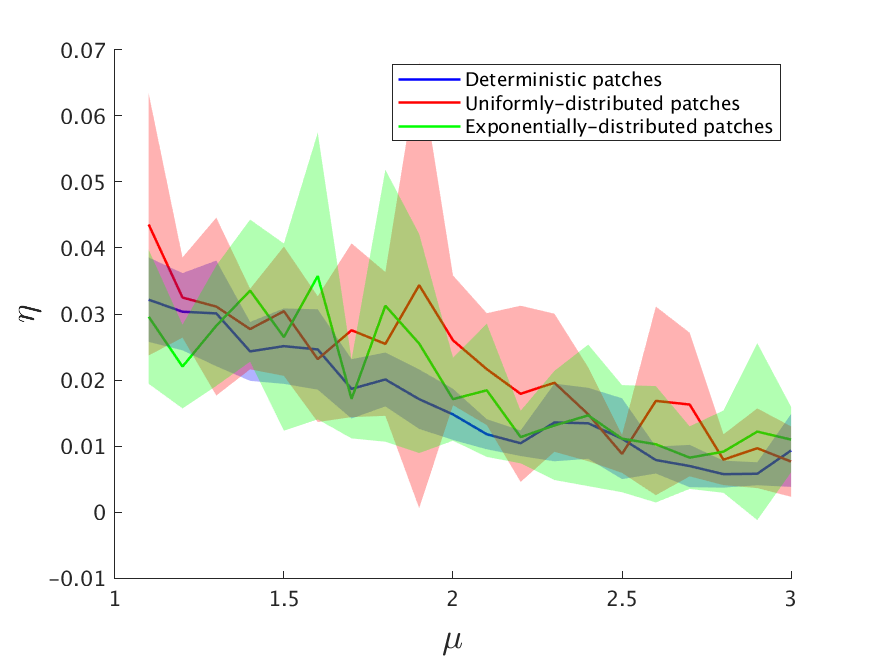
\includegraphics[width=.50\textwidth]{EffectOfTargetDist1D_D_PowerLaw_5found-10reps}\label{fig:EffectOfTargetDist1D_PowerLaw_D_base}}\hfill
	\subfloat[{$5$ targets found, repeated $50$ times}]{%
		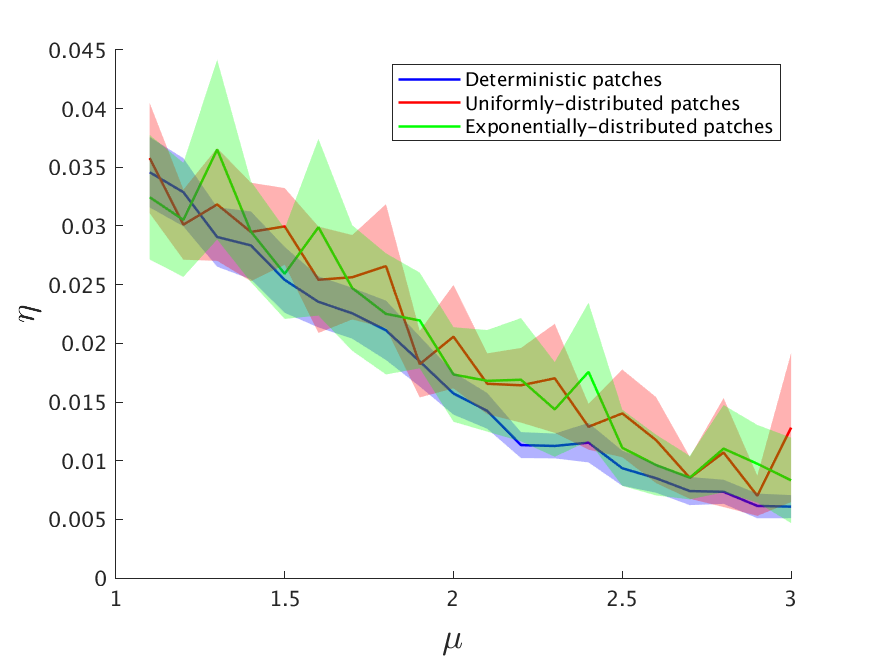
\includegraphics[width=.50\textwidth]{EffectOfTargetDist1D_D_PowerLaw_5found-50reps}\label{fig:EffectOfTargetDist1D_PowerLaw_D_morereps}}\\
	\subfloat[$50$ targets found, repeated $10$ times]{%
		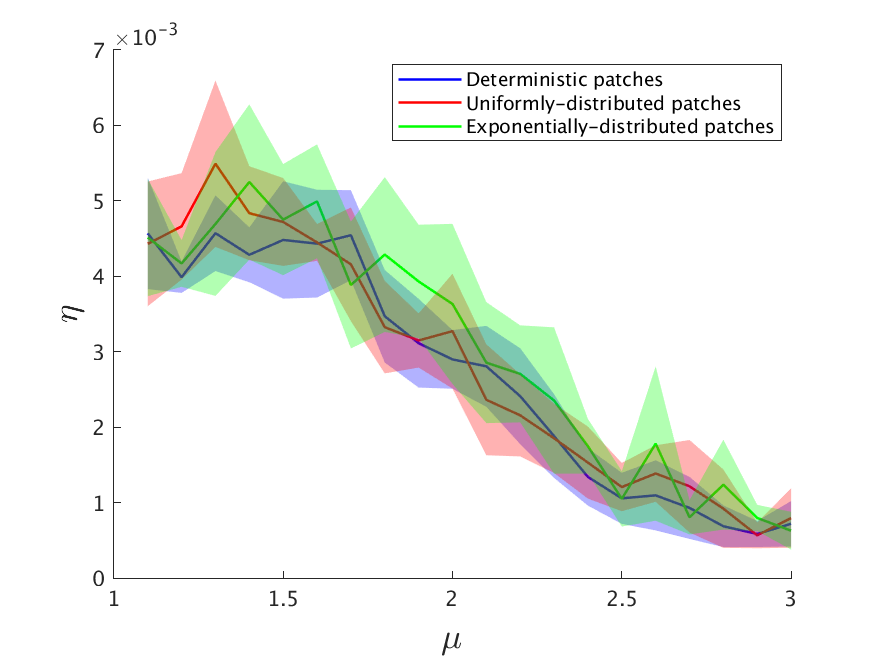
\includegraphics[width=.50\textwidth]{EffectOfTargetDist1D_D_PowerLaw_50found-10reps}\label{fig:EffectOfTargetDist1D_PowerLaw_D_morefound}}\hfill
	\subfloat[$50$ targets found, repeated $200$ times]{%
		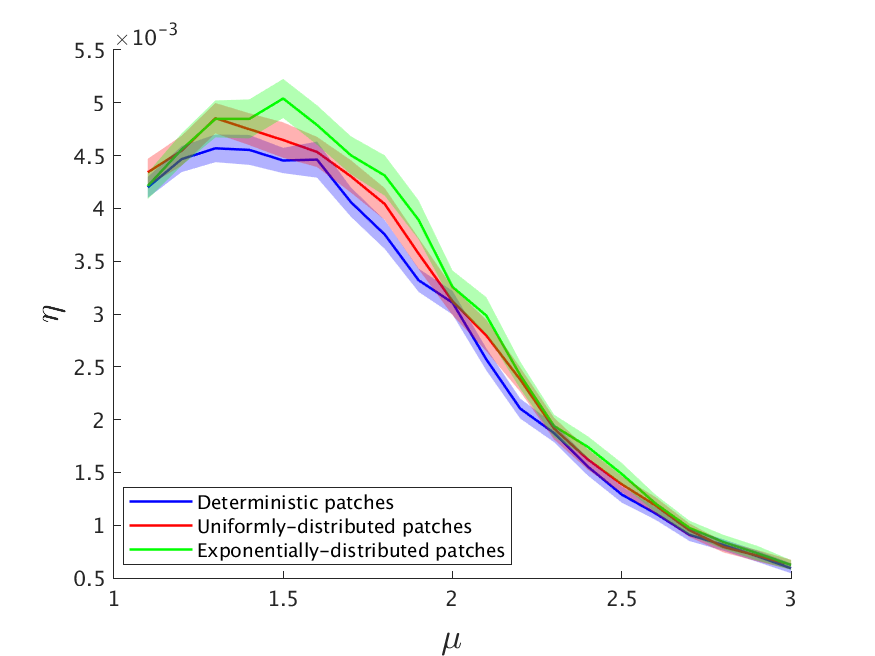
\includegraphics[width=.50\textwidth]{EffectOfTargetDist1D_D_PowerLaw_50found-200reps}\label{fig:EffectOfTargetDist1D_PowerLaw_D_moreboth}}
	\caption[Mean efficiency of an unbounded power-law strategy for three different target distributions for a different numbers of repetitions and targets to be found]{The mean efficiency of a random walk search strategy with a power-law step-length distribution, with parameter ranging from $1.1 \leq \mu \leq 3$ over $20$ equispaced values, for destructive foraging ($x_0=\lambda/2$) and with three different target distributions: deterministic, uniform, and exponential, each with an average distance between targets of $\lambda = 20$, and a radius of vision, $r_v=1$. Each subplot ran the simulation for a different number of repetitions and had a different requirement on the number of targets to find.}\label{fig:EffectOfTargetDist1D_PowerLaw_D}
\end{figure}

Looking first at \cref{fig:EffectOfTargetDist1D_PowerLaw_D_base}, there is clearly a large variance in the mean efficiency across values of $\mu$ for all target distributions. Comparing the distribution types across \cref{fig:EffectOfTargetDist1D_PowerLaw_D_base,fig:EffectOfTargetDist1D_PowerLaw_D_morefound,fig:EffectOfTargetDist1D_PowerLaw_D_morereps}, the exponentially distributed targets seem to have the biggest variance in efficiency, with the uniform and deterministic target distributions seeming to have similar variances to each other. 

The increase in the total targets found per search from \cref{fig:EffectOfTargetDist1D_PowerLaw_D_base} to \cref{fig:EffectOfTargetDist1D_PowerLaw_D_morefound} reduces the variances in our mean efficiency for all three target distributions, although there is still a large spike in the exponentially-distributed targets around $\mu\approx 1.6$. The increase from $5$ targets found to $50$ targets found also reduces the efficiency by a factor of $10$. The efficiency seems to be very similar, if not the same, for the three different target distributions. Similarly, increasing the total number of times that the simulation is repeated from \cref{fig:EffectOfTargetDist1D_PowerLaw_D_base} to \cref{fig:EffectOfTargetDist1D_PowerLaw_D_morereps} smooths out the mean efficiency. The two key differences between repeating more searches versus running longer (in terms of targets) searches, is that when a new search begins the forager is reset to a random point within the first interval, and the targets are regenerated. Whereas after a target is found the animal resumes searching from where it found the target, and the targets become more scarce over time. Increasing the number of targets found seems to have a larger effect on reducing the variance than increasing the number of repetitions. Longer searches are also a more realistic model of the real world, since animals are generally not reset to a new location with a new set of targets.


Finally, in \cref{fig:EffectOfTargetDist1D_PowerLaw_D_moreboth} the number of repetitions is large enough that the efficiency curves are smooth and the confidence intervals are narrow. For $\mu \approx 1$, the efficiency is very similar between distributions, but as $\mu$ increases there is a clear difference in the efficiency between different target distributions. For values of $\mu \approx 3$, there is little if any difference in the efficiency between different target distributions. Therefore, the efficiency of a L\'{e}vy search depends on the distribution of targets, and for ballistic and Brownian searches there is not necessarily a dependence on the target distribution. However, the efficiency only changes slightly between different distributions, and the curves follow roughly the same shape, with the peak efficiency for each curve occurring close to each other. There are analytic models in the literature that allow for different target distributions (e.g. \cite{Bartumeus_2013}), which we could potentially use to extend our model. 

Although the deterministic target assumption will potentially affect the optimal parameters of any search strategy we investigate, the amount of difference between the target distributions seems small enough to justify making the simplification, especially given the relatively large variance in efficiency across multiple searches.


\subsection{Comparing the two different measures of efficiency \label{sec:1D_assumptions:efficiency}}
At the start of \cref{sec:1Dmodel}, we made the claim that optimising the efficiency of a search over the real line was equivalent to optimising the efficiency in finding the first target, given known starting conditions (either $x_0 = r_v$ or $x_0 = \lambda/2$). This claim is made throughout the animal foraging literature (e.g. \cite{Bartumeus_2013}).

Intuitively, as more targets are found the search space becomes more sparse and so the efficiency will decrease, which should mean that the efficiency over multiple targets is less than that of finding a single target. This can also be seen in \cref{fig:EffectOfTargetDist1D_PowerLaw_D_base,fig:EffectOfTargetDist1D_PowerLaw_D_morefound,fig:EffectOfTargetDist1D_PowerLaw_D_morereps,fig:EffectOfTargetDist1D_PowerLaw_D_moreboth} in the previous section, where the efficiency changed depending on how many targets were required to be found throughout each search. The two measures of efficiency are clearly not going to be equal to each other, although our claim is that optimising for either definition is equivalent, meaning that the maximum efficiency under both definitions occurs at the same location.

We define the efficiency of a search that finds $N$ targets as
\begin{equation*}
\eta_N = \frac{N}{L}, 
\end{equation*}
where $L$ is the total distance travelled, and $N$ is the number of targets found throughout the search, where the subscript $N$ is used to make clear the dependence on the number of targets found.

Also recall the notion of efficiency used throughout \cref{sec:1Dmodel}, 
\begin{equation}
\label{eq:1d_assumptions:eta}
\eta = \frac{1}{\E{L}}.
\end{equation}
Note that under this definition of $\eta$, we are assuming a known starting point, as opposed to the $\eta_N$ definition which assumes a random starting location. For the remainder of this section we include the dependence on the starting location explicitly. For destructive foraging,
\begin{equation*}
\eta_{d} = \frac{1}{\E{L(\lambda/2)}},
\end{equation*}
where $L(x)$ represents the total distance to find a target for a search that begins at location $x$. For non-destructive foraging we have
\begin{equation*}
\eta_{n} = \frac{1}{\E{L(r_v)}}.
\end{equation*}
The first case to consider is when the targets are non-destructive. Consider the efficiency across finding $N$ targets, $\eta_N$, assuming that the forager starts at a random location between two targets, which may occur if we were to release an animal at random in some search space. Each time a target is reached, the animal begins its search a distance $r_v$ away from the target in either direction. Since all intervals are statistically equivalent, and due to the symmetry of the step-length distribution, we can without loss of generality assume that the animal continues its search for the next target at location $x_0 = r_v$ in the interval $[0,\lambda]$. The search for the first target is unique in that it can begin at any point in the interval, whereas the searches for each of the remaining $N-1$ targets must begin at the same point, or a statistically equivalent point, since all searches will begin $r_v$ from a target. If we define $L_i(r_v)$ as the distance travelled when finding the $i$th target, beginning from $x=r_v$, as , then we can say that $L_i(r_v)$ for $i \geq 2$ are independent and identically distributed. Using this notation, we may rewrite $\eta_N$ as
\begin{equation*}
\eta_N = \frac{N}{L_1(\lambda/2) + L_2(r_v) + \dots + L_N(r_v)}.
\end{equation*}
When $N$ is large, the random variable $L_1$ has a relatively small impact on the denominator, and so through the strong law of large numbers we know that
\begin{equation*}
\lim_{N \to \infty} \eta_N = \frac{1}{\E{L_2(r_v)}} \text{ a.s.}
\end{equation*}

That is, for a non-destructive search, the long-term efficiency is the reciprocal of the expected distance travelled in a single search that begins at $r_v$. This is the same as our definition of $\eta$. We can consider $\eta_N$ as the sample efficiency, which converges to $\eta$, the efficiency. In \cref{fig:EtaVsEtaN_PowerLaw_ND} we plot both $\eta$ and $\eta_N$ for a range of $N$ to further demonstrate this. The large $N$ gets, the closer $\eta_N$ gets to $\eta$.

\begin{figure}[h!]
	\centering
	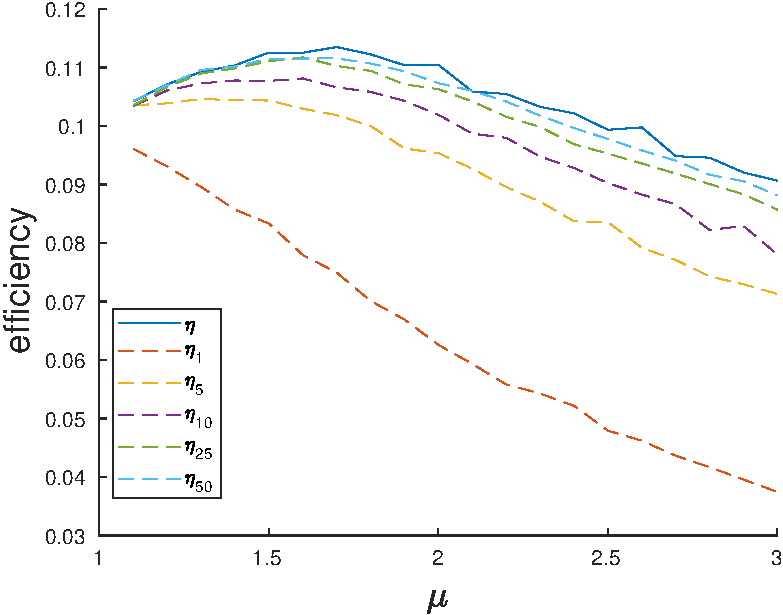
\includegraphics[scale=0.68]{EtaVsEtaN_PowerLaw_ND_reps5000}
	\caption[Two different definitions of the efficiency, $\eta$ and $\eta_N$, compared to each other for non-destructive foraging]{The efficiency, $\eta$, as defined in \cref{eq:1d_assumptions:eta} versus $\eta_N$ plotted for a range of search lengths, $N=\{1,5,10,25,50\}$, for non-destructive foraging ($x_0 = r_v$ for $\eta$ calculation) with $\lambda=20$, $r_v=1$, and $\lmin = 1$. Efficiency is averaged over $5000$ simulations. The larger $N$ is, the closer $\eta_N$ is to $\eta$. \label{fig:EtaVsEtaN_PowerLaw_ND}}
\end{figure}


For the case of destructive foraging, an analytic argument is not as simple because as targets get more sparse, the starting location of the forager will depend on which targets have been destroyed. Instead, we simulate $\eta_N$ and $\eta$ for the destructive foraging case in \cref{fig:EtaVsEtaN_PowerLaw_D}. Although $\eta_N$ is clearly different to $\eta$, and there does not seem to be convergence as $N$ increases, we can still note that the peak efficiency occurs at the same location for both $\eta$ and $\eta_N$.

\begin{figure}[h!]
	\centering
	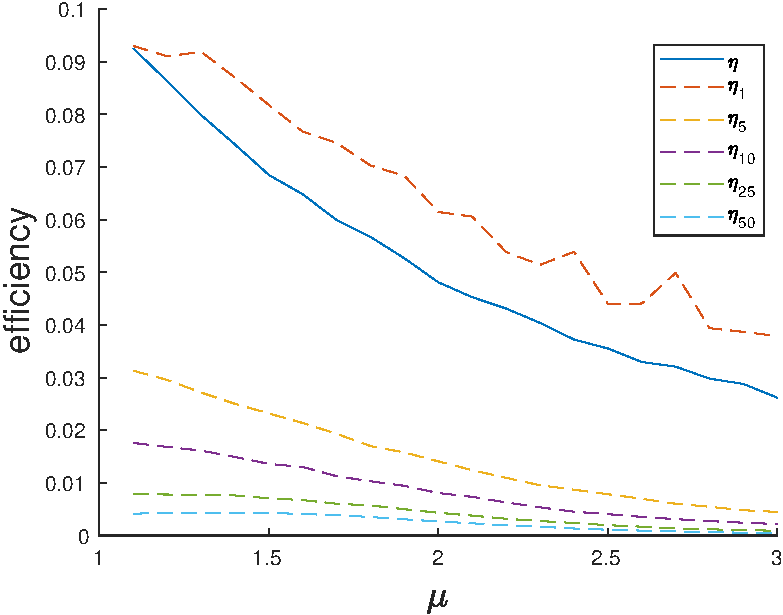
\includegraphics[scale=0.68]{EtaVsEtaN_PowerLaw_D_reps500}
	\caption[Two different definitions of the efficiency, $\eta$ and $\eta_N$, compared to each other for non-destructive foraging]{The efficiency, $\eta$, as defined in \cref{eq:1d_assumptions:eta} versus $\eta_N$ plotted for a range of search lengths, $N=\{1,5,10,25,50\}$, for destructive foraging ($x_0 =\lambda/2$ for $\eta$ calculation) with $\lambda=20$, $r_v=1$, and $\lmin = 1$. Efficiency is averaged over $5000$ simulations. The only difference between $\eta$ and $\eta_1$ is that the former begins at $x_0=\lambda/2$ whereas the latter begins at a uniformly distributed location within $[0,\lambda]$. \label{fig:EtaVsEtaN_PowerLaw_D}}
\end{figure}
